\section*{Organisatorisches}

	\begin{frame}
		\frametitle{Kontakt}
		\begin{tabular}{ll}
			Anschrift & Technische Universität Dortmund\\
			& Lehrstuhl für Förder- und Lagerwesen (FLW)\\
			& LogistikCampus\\
			& Joseph-von-Fraunhofer-Str. 2-4 \\
			& 44227 Dortmund\\[0.1cm]
			Name & Mojtaba MasoudiNejad, M.Sc.\\[0.1cm]
			Raum& A4.06\\[0.1cm]
			Telefon& +49 231 755-3236\\[0.1cm]
			Mail& mojtaba.masoudinejad@tu-dortmund.de\\[0.1cm]
			Sprechstunde& flexibel nach Vereinbarung\\[0.1cm]
		\end{tabular}
	\end{frame}

	\begin{frame}
		\frametitle{Master Präsentation Termine}
		\begin{tabular}{ll}
		Ort & FLW / A3.16\\[0.1cm]
		Zeit & 18 Oct. 2019 um 11:00 - 11:25 \\[0.1cm]
		Examiners &  Moritz Roidl, Dipl.-Inform.\\
		&Mojtaba MasoudiNejad, M.Sc.
		\end{tabular}\\[1cm]
	\end{frame}

	\begin{frame}
	\frametitle{Literatur}
	    \begin{columns}[T]
	        \begin{column}{0.49\textwidth}
	            \begin{itemize}%[<+->] Kommentar entfernen falls jeder Punkt einzeln erscheinen soll
					\item Title: Springer Handbook of Robotics
					\item Author: Khatib, Oussama ; Siciliano, Bruno
					\item Link: \href{https://www.ub.tu-dortmund.de/katalog/titel/HT019024543}{https://www.ub.tu-dortmund.de/katalog/titel/HT019024543}
	        	\end{itemize}
	        \end{column}
	        \begin{column}{0.49\textwidth}
	        	\centering
	            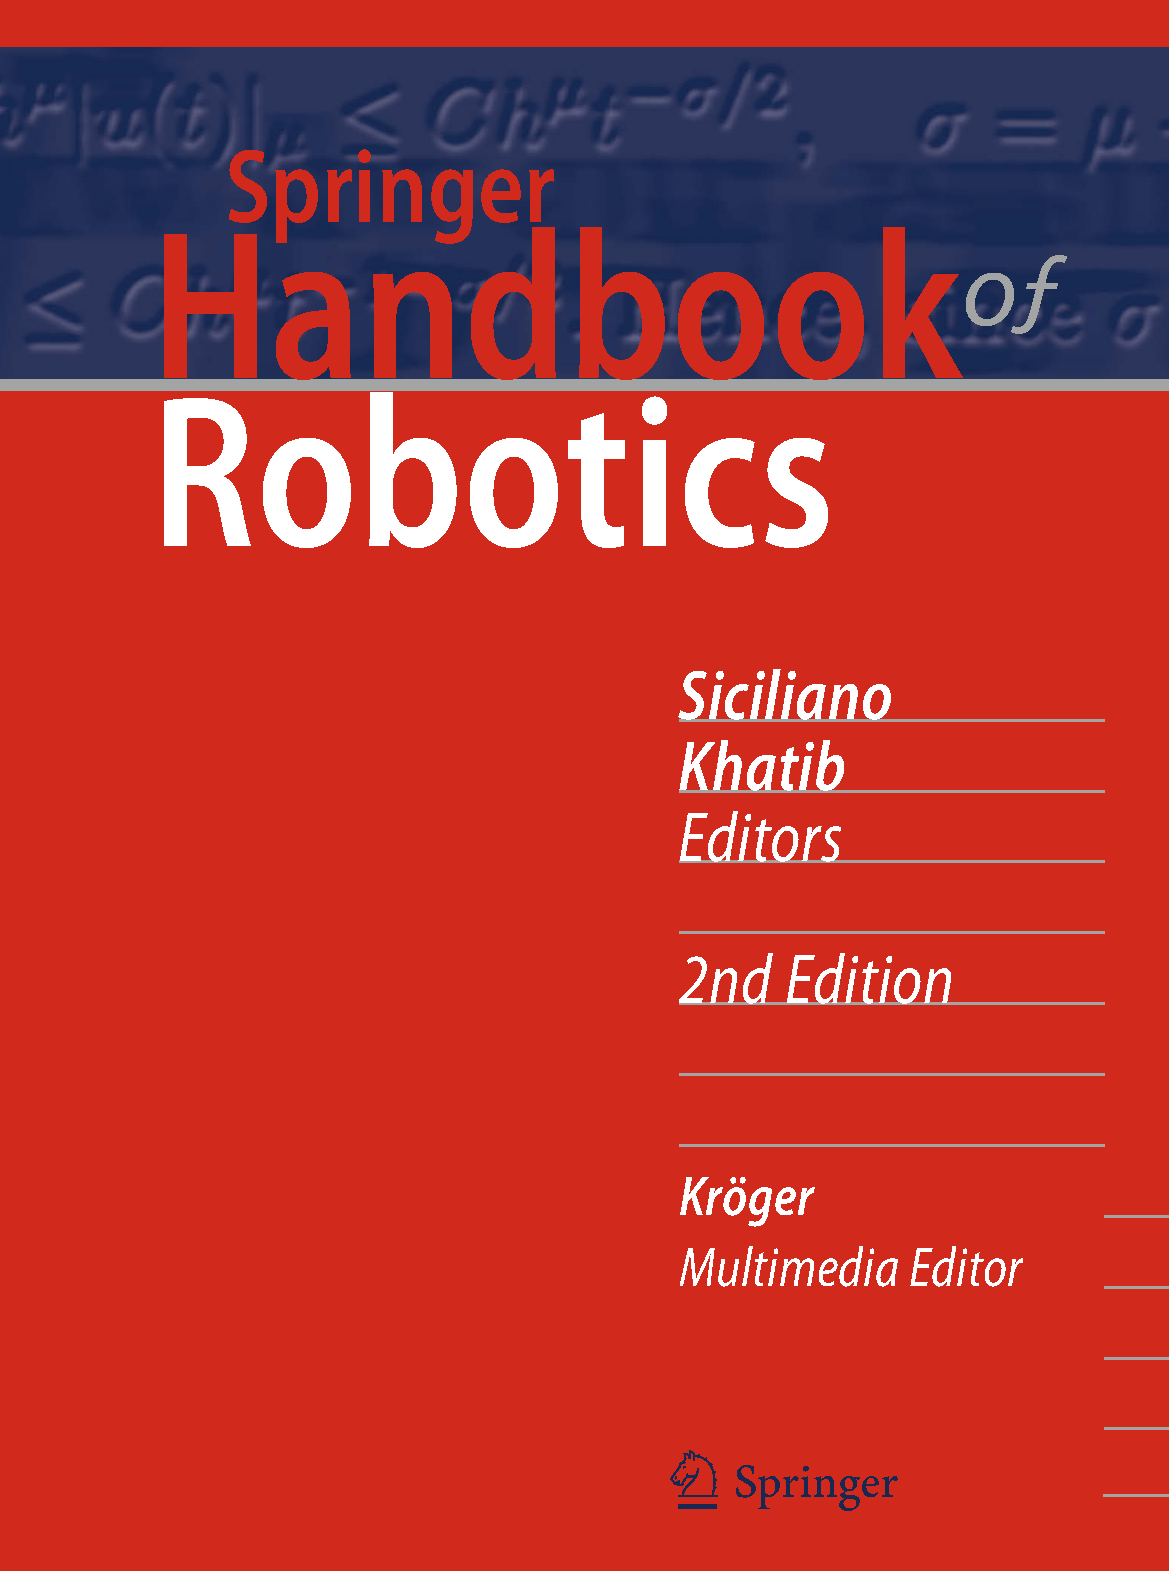
\includegraphics[scale=0.25]{pictures/springer_robotics.pdf}
	        \end{column}
	    \end{columns}
	\end{frame}

	\begin{frame}
		\frametitle{Literatur}
		\begin{columns}[T]
			\begin{column}{0.49\textwidth}
				\begin{itemize}%[<+->] Kommentar entfernen falls jeder Punkt einzeln erscheinen soll
					\item Title: Model Predictive Control : Theory, Computation, and Design 
					\item Author: Diehl, Moritz ; Mayne, David Q ; Rawlings, James Blake
					\item Link: \href{https://www.ub.tu-dortmund.de/katalog/titel/HT019602243}{https://www.ub.tu-dortmund.de/katalog/titel/HT019602243}
				\end{itemize}
			\end{column}
			\begin{column}{0.49\textwidth}
				\centering
				\includegraphics[scale=0.305]{pictures/mpc_book_cover.png}
			\end{column}
		\end{columns}
	\end{frame}

	\begin{frame}
		\frametitle{Literatur}
		\begin{columns}[T]
			\begin{column}{0.49\textwidth}
				\begin{itemize}%[<+->] Kommentar entfernen falls jeder Punkt einzeln erscheinen soll
					\item Title: Numerical Optimization
					\item Author: Nocedal, Jorge ; Wright, Stephen J
					\item Link: \href{https://www.ub.tu-dortmund.de/katalog/titel/HT014641035}{https://www.ub.tu-dortmund.de/katalog/titel/HT014641035}
				\end{itemize}
			\end{column}
			\begin{column}{0.49\textwidth}
				\centering
				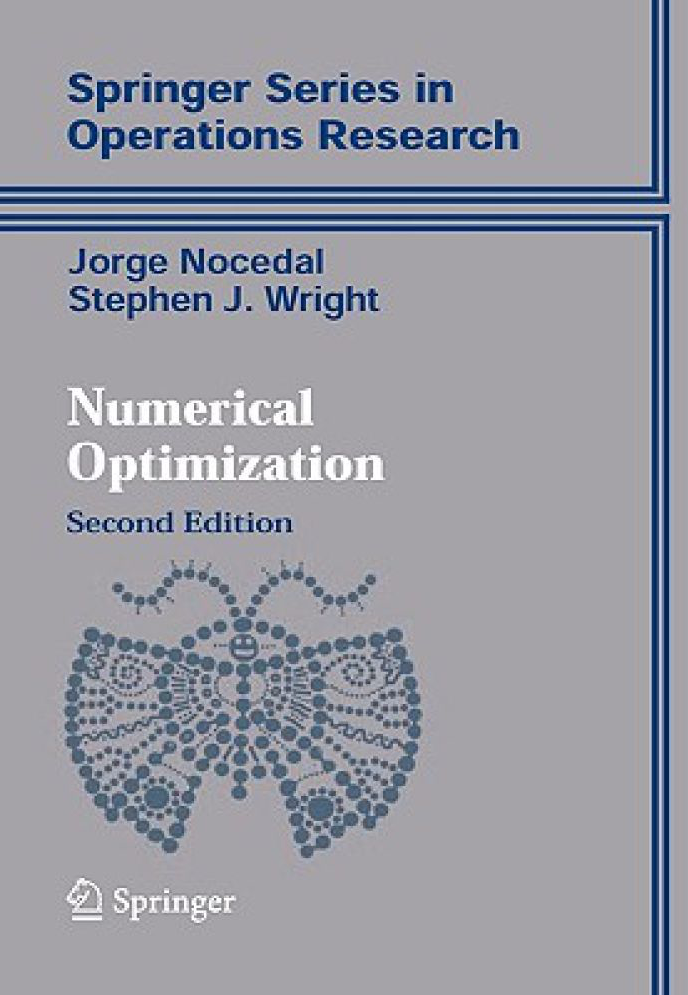
\includegraphics[scale=0.2]{pictures/numerical_optimization.png}
			\end{column}
		\end{columns}
	\end{frame}